%%% Local Variables: 
%%% coding: utf-8
%%% mode: latex
%%% TeX-engine: xetex
%%% End: 

\documentclass[hide notes,intlimits]{beamer}

\mode<presentation>
{
  \usetheme{PISMshade}
  \setbeamercovered{transparent}
}

% load packages
\usepackage{media9}
\usepackage[english]{babel}
\usepackage[multidot]{grffile}

\usepackage{tikz}
\usetikzlibrary{shapes,arrows}
\usetikzlibrary{shadows}

\definecolor{dark red}{HTML}{E41A1C}
\definecolor{dark green}{HTML}{4DAF4A}
\definecolor{dark violet}{HTML}{984EA3}
\definecolor{dark blue}{HTML}{084594}
\definecolor{dark orange}{HTML}{FF7F00}
\definecolor{light blue}{HTML}{377EB8}
\definecolor{light red}{HTML}{FB9A99}
\definecolor{light violet}{HTML}{CAB2D6}

\setbeamercolor{boxed}{fg=black,bg=light blue!25}
\graphicspath{{figures/}{../figures/}{../figures_2018_08/}{../2021_09_cph/figures/}}

\newenvironment{transbox}[1][]{%
\begin{tikzpicture}
\node[drop shadow,rounded corners,text width=.9\textwidth,fill=white, fill opacity=#1,text opacity=1] \bgroup
}{
\egroup;\end{tikzpicture}} 

\newenvironment{transbox-tight}{%
\begin{tikzpicture}
\node[drop shadow,rounded corners,fill=uaf yellow, fill opacity=0.75,text opacity=1] \bgroup
}{
\egroup;\end{tikzpicture}} 

\newcommand{\jl}{[\![}
\newcommand{\jr}{]\!\hskip 0.003cm ]}
\newcommand{\bpsi}{\boldsymbol{\psi}}
\newcommand{\bPsi}{\boldsymbol{\Psi}}
\newcommand{\bphi}{\boldsymbol{\phi}}
\newcommand{\bPhi}{\boldsymbol{\Phi}}
\newcommand{\bn}{\mathbf{n}}
\newcommand{\bq}{\mathbf{q}}
\newcommand{\bv}{\mathbf{v}}
\newcommand{\D}{\,\mathrm{d}}
\newcommand{\Tsnow}{T_{\text{snow}}}
\newcommand{\Hatm}{H_{\text l}^{\text{atm}}}

\newcommand{\mathtext}[1]{\mathsf{#1}}

% title page
\title[Ice sheet modeling] % (optional, use only with long paper titles)
{Towards credible projections of sea-level rise}

\author[Aschwanden] % (optional, use only with lots of authors)
{\textbf{Andy Aschwanden}, D. Brinkerhoff}
\institute{Geophysical Institute, University of Alaska Fairbanks}

% - Give the names in the same order as the appear in the paper.
% - Use the \inst{?} command only if the authors have different
%   affiliation.

% - Use the \inst command only if there are several affiliations.
% - Keep it simple, no one is interested in your street address.

% \titlegraphic{\vskip-1.cm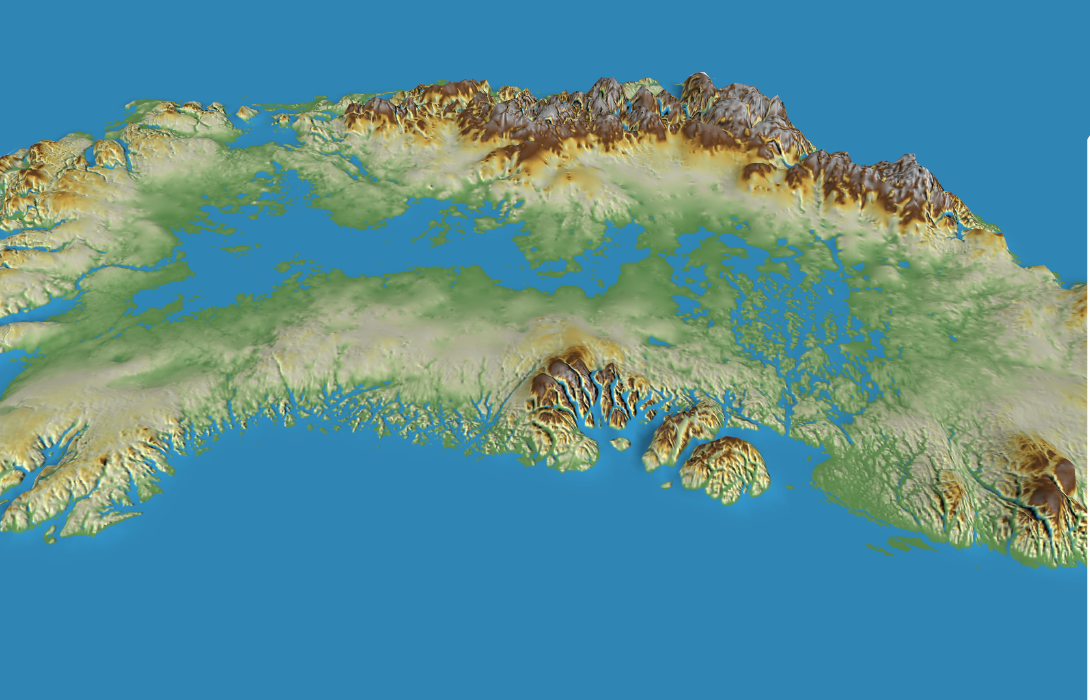
\includegraphics[height=3.5cm]{gris-green-collage-clean}}

\date{}


\subject{The Greenland Ice Sheet}

\begin{document}


\setbeamertemplate{background canvas}
  {
     \tikz{\node[inner sep=0pt,opacity=1.0] {\includegraphics[width=\paperwidth]{uaf_beamer_shade_bg}};}
} 

% insert titlepage
\begin{frame}
  \titlepage
  \note[item]{Collaboration Martin, Doug}
\end{frame}


%% \setbeamertemplate{background canvas}
%%   {
%%      \tikz{\node[inner sep=0pt,opacity=1] {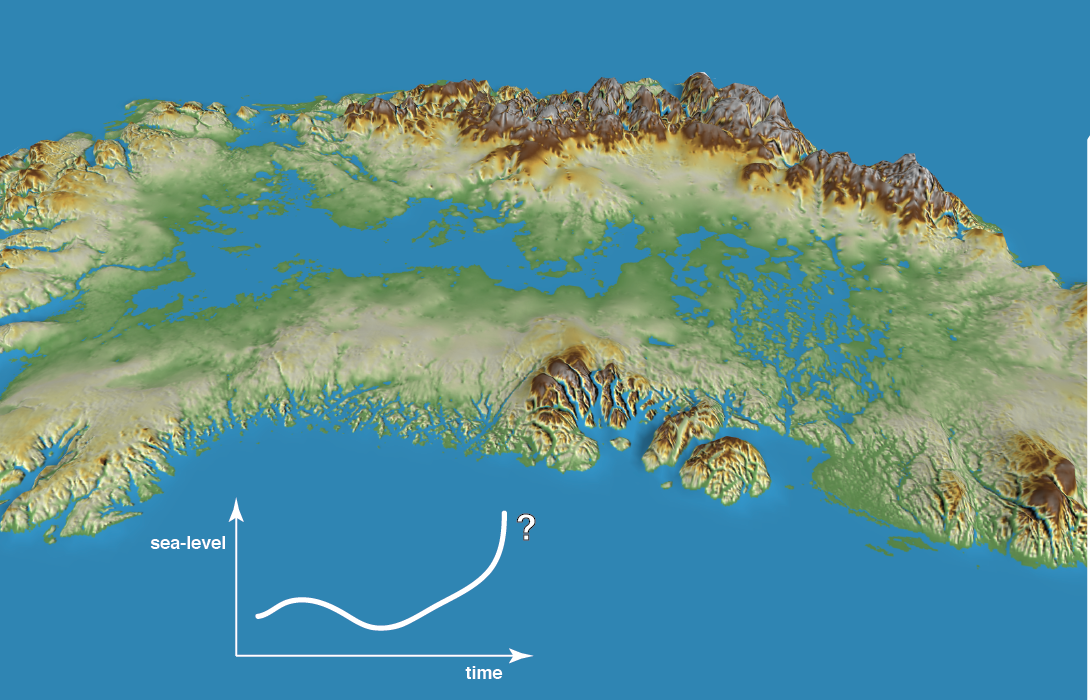
\includegraphics[height=\paperheight,width=\paperwidth]{gris-green-collage-slr}};}
%% } 


\setbeamertemplate{background canvas}
{
%
}

\begin{frame}{Modern sea-level change}
  \begin{figure}
    \includegraphics<1>[width=\textwidth]{sea-level-from-altimetry}
  \end{figure}
\end{frame}

\begin{frame}{Modern and projected mass loss from Greenland}
  \begin{figure}
    \includegraphics<1>[width=\textwidth]{ar6-fig17-no-zoom}
    \includegraphics<2>[width=\textwidth]{ar6-fig17-with-zoom}
  \end{figure}
\end{frame}

\begin{frame}{Modern and projected Arctic sea ice extend}
  \begin{figure}
    \includegraphics<1>[width=\textwidth]{grl23061-fig-0001}
  \end{figure}
\end{frame}



\begin{frame}{A simulation made in 2010}
  \begin{figure}
    \includegraphics[width=0.65\textwidth]{gris-obs-exp-old}
    \caption{Observed and simulated surface speeds in meters per year}
  \end{figure}
\end{frame}

\begin{frame}{A simulation made in 2016}
  \begin{figure}
    \includegraphics[width=0.65\textwidth]{gris-obs-exp-new}
    \caption{Observed and simulated surface speeds in meters per year}
  \end{figure}
\end{frame}


%% \begin{frame}{AS19 Projections}
%%   \begin{figure}
%%     \includegraphics[width=0.9\textwidth]{projection_as19}
%%   \end{figure}
%% \begin{itemize}
%% \item 500 member ensemble to assess parametric uncertainty
%% \item all scenarios show large variance, which is a feature not a bug
%% \end{itemize}
%% \note[item]{}
%% \end{frame}


%% \begin{frame}{Limitations of AS19 and ISMIP6}
%%   \begin{figure}
%%     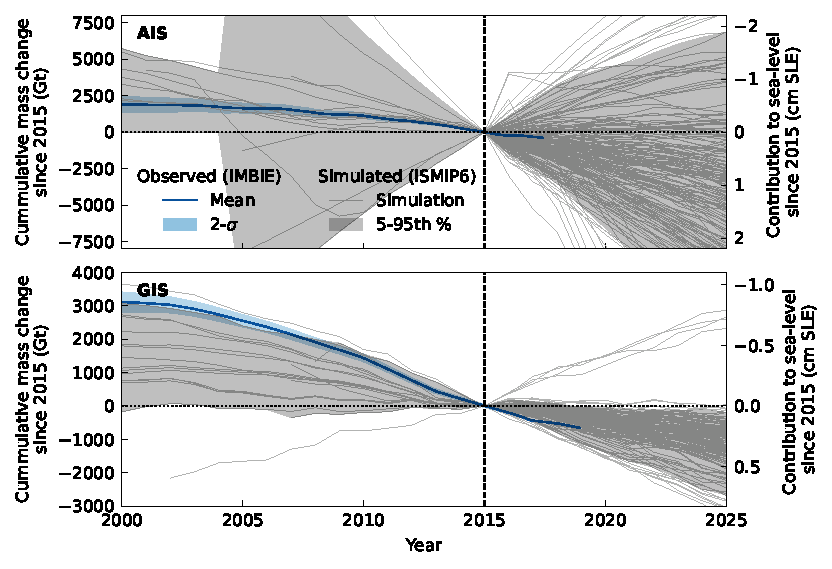
\includegraphics[width=0.75\textwidth]{IS_historical}
%%   \end{figure}
%% \begin{itemize}
%% \item AS19 did prior calibration and literature values to define probability distributions of parameters \alert{but}
%% \item did \alert{NOT} excplicitly condition on observations
%% \item see our commentary in TCD (in revision)
%% \end{itemize}
%% \note[item]{}
%% \end{frame}

%% \begin{frame}{2-step calibration}
%% Which quantities should we use?
%% \begin{itemize}
%% \item use the quantity of interest: mass change
%% \item use quantity that contributes a lot to uncertainty: ice flow
%% \end{itemize}
%% \note[item]{}
%% \end{frame}

%% \begin{frame}{1. Ice Flow: calibrate parameters}
%% \begin{itemize}
%% \item use Markov Chain Monte Carlo sampling to find the joint distribution of these parameters.
%% \item think of PISM as a map $\mathcal{F}$ from a parameter vector $\mathbf{x}$ to surface speeds $\mathbf{Y}$
%% \begin{equation}
%% \mathbf{Y} = \mathcal{F}(\mathbf{x})
%% \end{equation}
%% \item running the forward model (PISM) is too expensive for MCMC
%% \item Generate a ``cheap'' surrogate model $\mathcal{G}$ such that
%% \begin{equation}
%% \mathcal{G}(\mathbf{x}) \approx \mathcal{F}(\mathbf{x})
%% \end{equation}
%% \end{itemize}

%%   \note[item]{We take a Bayesian approach and use Markov Chain Monte Carlo sampling to find the joint distribution of these parameters.  While this problem is computationally challenging due to the significant expense of running the forward model, we made it tractable by employing a neural-network based surrogate model that provides a low-cost mapping from parameters to velocity fields \citep{Brinkerhoff2020}.}
%% \end{frame}

%% \begin{frame}{1. Ice Flow: training data}
%% \begin{itemize}
%% \item select 8 relevant parameters
%% \item define a prior probability distribution for each parameter
%% \item draw 1,000 samples using Sobol Sequences
%% \item run PISM 1,000 times
%% \end{itemize}
%% \end{frame}

%% \begin{frame}{1. Ice Flow: Surrogate model}
%% \begin{itemize}
%% \item use 4 layer Neural Network surrogate model by Brinkerhoff et al (2021)
%% \item implemented in PyTorch
%% \item train surrogate model on NVIDIA GPU
%% \end{itemize}
%% \end{frame}




%% \begin{frame}{Challenge $\mathbf{Y}$ is not a scalar}
%% Compared to e.g., Hill (2021), Edwards (2019, 2021), etc, our $\mathbf{Y}$ is \alert{not} a scalar:
%% \begin{eqnarray}
%% \mathbf{x} = \{x_1, x_2,\ldots,x_n\}, & n = 8, \\ 
%% \mathbf{Y} = \{Y_1, Y_2, \ldots,Y_m \},& m \ge 10^6
%% \end{eqnarray}
%%   \note[item]{}
%% \end{frame}

%% \begin{frame}{Solution: dimensionality reduction using PCA}
%% \begin{itemize}
%% \item decompose training data into ``eigen-glaciers'' using Pricipal Component Analysis (``eigen faces'' in picture analysis)
%% \item we only need to simulate the first $\sim$50 eigen-coefficients to capture 99.95\% of the variance
%% \item we have reduce the problem from 10$^6$ to $\sim$50 unknowns.
%% \end{itemize}
%% \end{frame}


%% \begin{frame}{Calibrated Projections}
%%   \begin{figure}
%%     \includegraphics<1>[width=0.75\textwidth]{projection_as19}
%%     \includegraphics<2>[width=0.75\textwidth]{projection_flow}
%%     \includegraphics<3>[width=0.75\textwidth]{projection_flowmass}
%%     \includegraphics<4>[width=0.75\textwidth]{projection_bars}
%%   \end{figure}
%% \end{frame}

\end{document}
